This  design  requires   three   different  voltage  levels  (known  as  voltage
\emph{rails}),  which  are  \SI{28}{\volt},  \SI{5}{\volt}  and  \SI{3.3}{\volt}
respecitvely. Each rail has  different  requirements  as far as noise, power and
efficiency goes.

A  decision  for  each  voltage rail must be made. Do we use a switch-mode power
regulator  or a linear regulator?  The  general  trade-off  is  that  swith-mode
regulators have  a  very  high  efficiency,  but  due  to the nature of how they
transform voltages, they produce a lot more jitter on the output. In contrast, a
linear regulator produces almost  no jitter -- in fact, it even dampens incoming
jitter  by  a substantial amount -- however, the linear regulator has very  poor
efficiency since  it  just  ``burns''  the  excess voltage and produces a lot of
heat,  making  it  a  poor  candidate  for transforming between  larger  voltage
differences.

The \SI{28}{\volt} rail is already given, since that's precisely the voltage the
external power supply provides.

Seeing as there  is  a  very large voltage difference between \SI{28}{\volt} and
the next lower rail, \SI{5}{\volt}, we opted for  a  switch-mode  regulator, the
\emph{LT3973}, for efficiency reasons. The circuit 

All   digital   circuitry,   such  as  the   micro   controller,   operates   at
\SI{3.3}{\volt}. It  is  particularly  important for the \SI{3.3}{\volt} rail to
have as little noise/jitter as possible. This requirement  stems  from  the fact
that  the  analog-to-digital   (ADC)  conversions  and  digital-to-analog  (DAC)
conversions derive  their  reference  voltage from the \SI{3.3}{\volt} rail. Any
noise on  this  rail  could  impact  the accuracy of these conversions and could
result in  lower  accuracy  of the final, regulated output voltage of the device
itself. 

\begin{figure}[th!]
    \center
    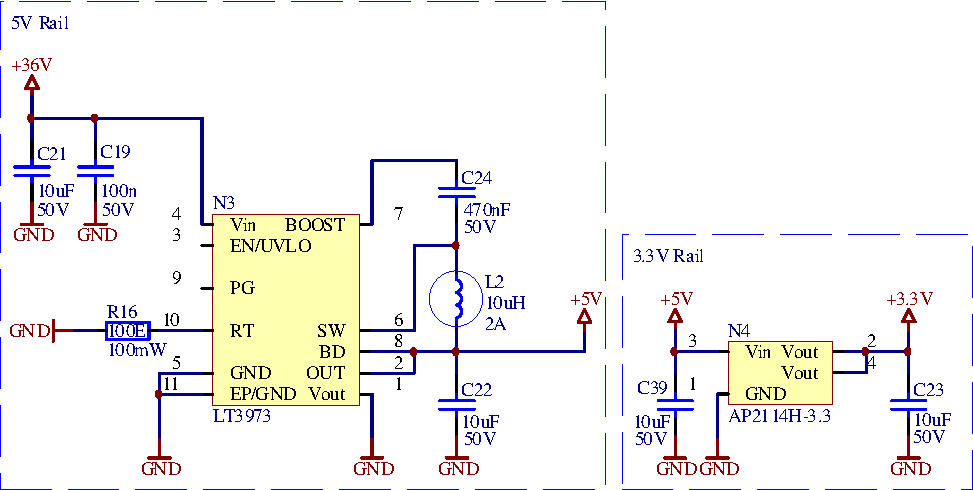
\includegraphics[width=.75\textwidth]{images/circuit/5v-3v-rails.pdf}
    \caption{Speisung f\"ur 5V mittels Abwertswandler (links) und Speisung f\"ur 3.3V mittels Linearregler (rechts)}
    \label{fig:circuit:rails}
\end{figure}

In a nutshell, in order to generate these voltage rails, the \SI{28}{\volt} from the
external power  supply  are  transformed  to  \SI{5}{\volt} by means of a buck
converter (switching step-down converter) and the \SI{3.3}{\volt} rail is generated by further reducing

Given that there is a significant difference in voltage (\SI{28}{\volt} to \SI{5}{\volt}), the use of a linear regulator would

Die  \SI{36}{\volt} vom Netzteil werden mittels eines getakteten  DC-DC-Wandlers
auf \SI{5}{\volt} transformiert,  was  in  der Abbildung \ref{fig:circuit:rails}
vom Bauteil $N_3$ verwirklicht wird.

Die  \SI{5}{\volt}  werden  von  einem  Linearregler  $N_4$ auf  \SI{3.3}{\volt}
gestuft. Ein Linearregler wurde  gew\"ahlt  damit  die  \SI{3.3}{\volt} Speisung
m\"oglichst  St\"orfrei  bleibt  --  Getaktete  Wandler  verursachen  viel  mehr
St\"orung. Somit  wird  verhindert,  dass  die DACs und ADCs verrauscht sind und
ungenau messen.

